\chapter{From Threats to Solutions: A Literature Review of Wheat Disease Classification in Smart Agriculture}


\section{Introduction}
Wheat is a vital global crop but faces significant threats from fungal diseases, insect pests, and environmental stressors, leading to major yield losses. Traditional identification methods are often manual, slow, and dependent on expert knowledge, making them ineffective at scale. In contrast, recent advances in smart agriculture have introduced image-based approaches powered by deep learning. These methods analyze visual symptoms on wheat leaves, stems, or spikes using computer vision, offering accurate and scalable solutions for real-time disease detection.

This chapter reviews both the biological threats to wheat production and the image-based technologies used to address them. It outlines common diseases and pests, highlights deep learning-based classification methods, and discusses data collection, preprocessing, and model performance. Finally, it identifies current limitations and research gaps to support the development of more effective disease monitoring systems in precision agriculture.

\section{Motivation for the protection of wheat crops}

Wheat is an ancient and vital food crop that provides energy and feeds billions of people around the world (see Figure~\ref{fig:Figure001}). Its demand is growing quickly because it’s used in many affordable food products and plays a big role in global food security. The \gls{abb:fao} estimates that by 2050, the world will need about 840 million tonnes of wheat, up from 642 million tonnes today \parencite{sharma2015wheat}. This doesn’t even include the extra needs like animal feed or the impact of climate change.

The global importance of wheat is further reflected in its massive export volumes, with leading producers shipping tens of millions of tonnes annually (see Table~\ref{tab:wheat_exports_2022}), demonstrating its critical role in both domestic consumption and international food supply chains. To meet the growing demand, developing countries need to increase wheat production by 77\%, mostly by improving how much wheat is grown on the same land \parencite{sharma2015wheat}.  But this is becoming harder, as wheat productivity is slowing down and diseases are becoming a bigger problem. If we don’t manage pests and diseases properly, wheat production could fall short of what the world needs. It’s important to invest in research, use better farming methods, and grow disease-resistant wheat. Protecting this essential crop is key to making sure we have enough food for the future.


\begin{table}[ht]
\centering
\caption{Top 10 Countries Exporting the Most Wheat (2022) \parencite{wprWheatExports}}
\begin{tabular}{|l|r|}
\hline
\textbf{Country} & \textbf{Wheat Exports 2022 (T)} \\
\hline
Australia  & 28.8M \\
United States & 20.9M \\
France & 20.2M \\
Canada & 18.5M \\
Russia & 17.8M \\
Argentina & 12.9M \\
Ukraine & 11.2M \\
India & 6.8M \\
Kazakhstan & 6.3M \\
Germany & 6.2M \\
\hline
\end{tabular}
\label{tab:wheat_exports_2022}
\end{table}

\begin{figure}[H]
    \centering
    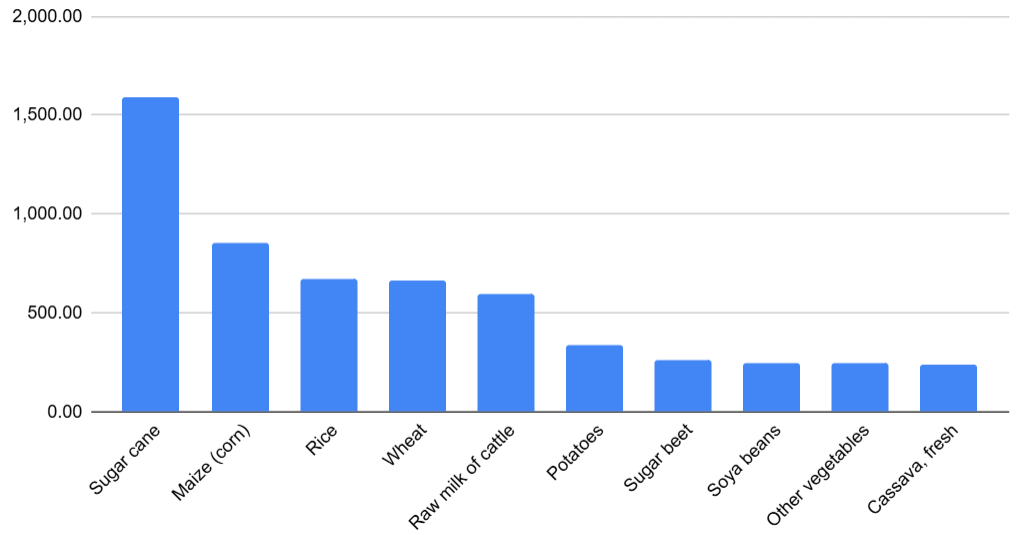
\includegraphics[width=0.9\textwidth]{chapters/chapter2/images/CropsProduction.png}
    \caption{Most Produced Commodities Worldwide in 2023 (in Million Tonnes) \parencite{faostat} }
    \label{fig:Figure001}
\end{figure}

The significance of wheat is also evident in its production across Arabic speaking nations, As shown in the figure ~\ref{fig:Alg} below, with Algeria ranking as the second-largest producer at 7 million tonnes per year, just behind Egypt (9.5 million tonnes). While this output is significant, production could increase even further by adopting modern farming techniques like the integrating of smart agriculture solutions.

\begin{figure}[H]
    \centering
    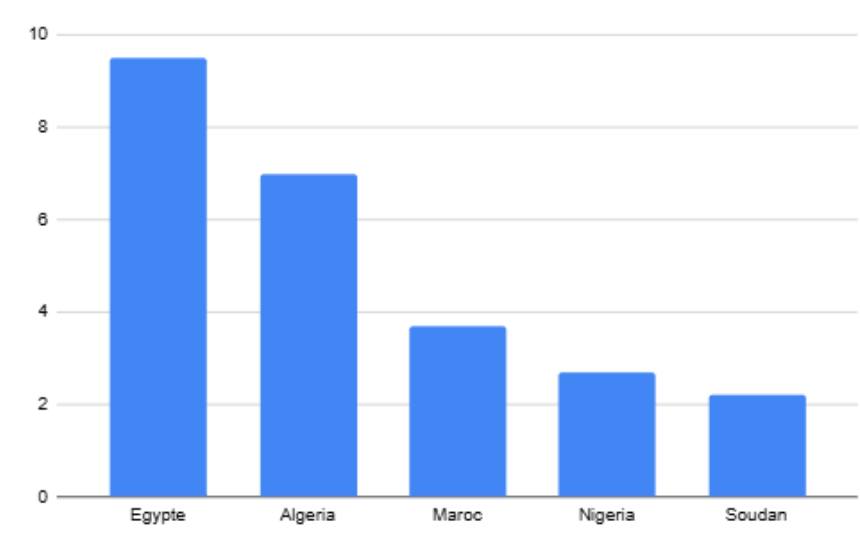
\includegraphics[width=0.8\textwidth]{chapters/chapter2/images/AlgeriaWheat.png}
    \caption{ Main African wheat producers in 2022/2023 (in Million Tonnes)\parencite{tadamsa2024} }
    \label{fig:Alg}
\end{figure}


\section{Wheat diseases: types and impacts}

Wheat diseases are influenced by several factors, including plant resistance, spore density, temperature, and environmental conditions, especially the presence of moisture on plant surfaces, which facilitates infection. While some fungi are host-specific, others can infect a wide range of plants. Symptoms can differ greatly, making accurate identification essential. Researchers primarily rely on fungal morphology for diagnosis. A clear understanding of these diseases is key to effective management and control \protect\parencite{haider2021wheat}. The following classification (Figure~\ref{fig:Figure02}) outlines the major wheat diseases, grouped by their causes and the plant parts they affect. Representative symptoms of these fungal diseases are illustrated in Figure~\ref{fig:wheat-diseases}.

\begin{figure}[H]
    \centering
    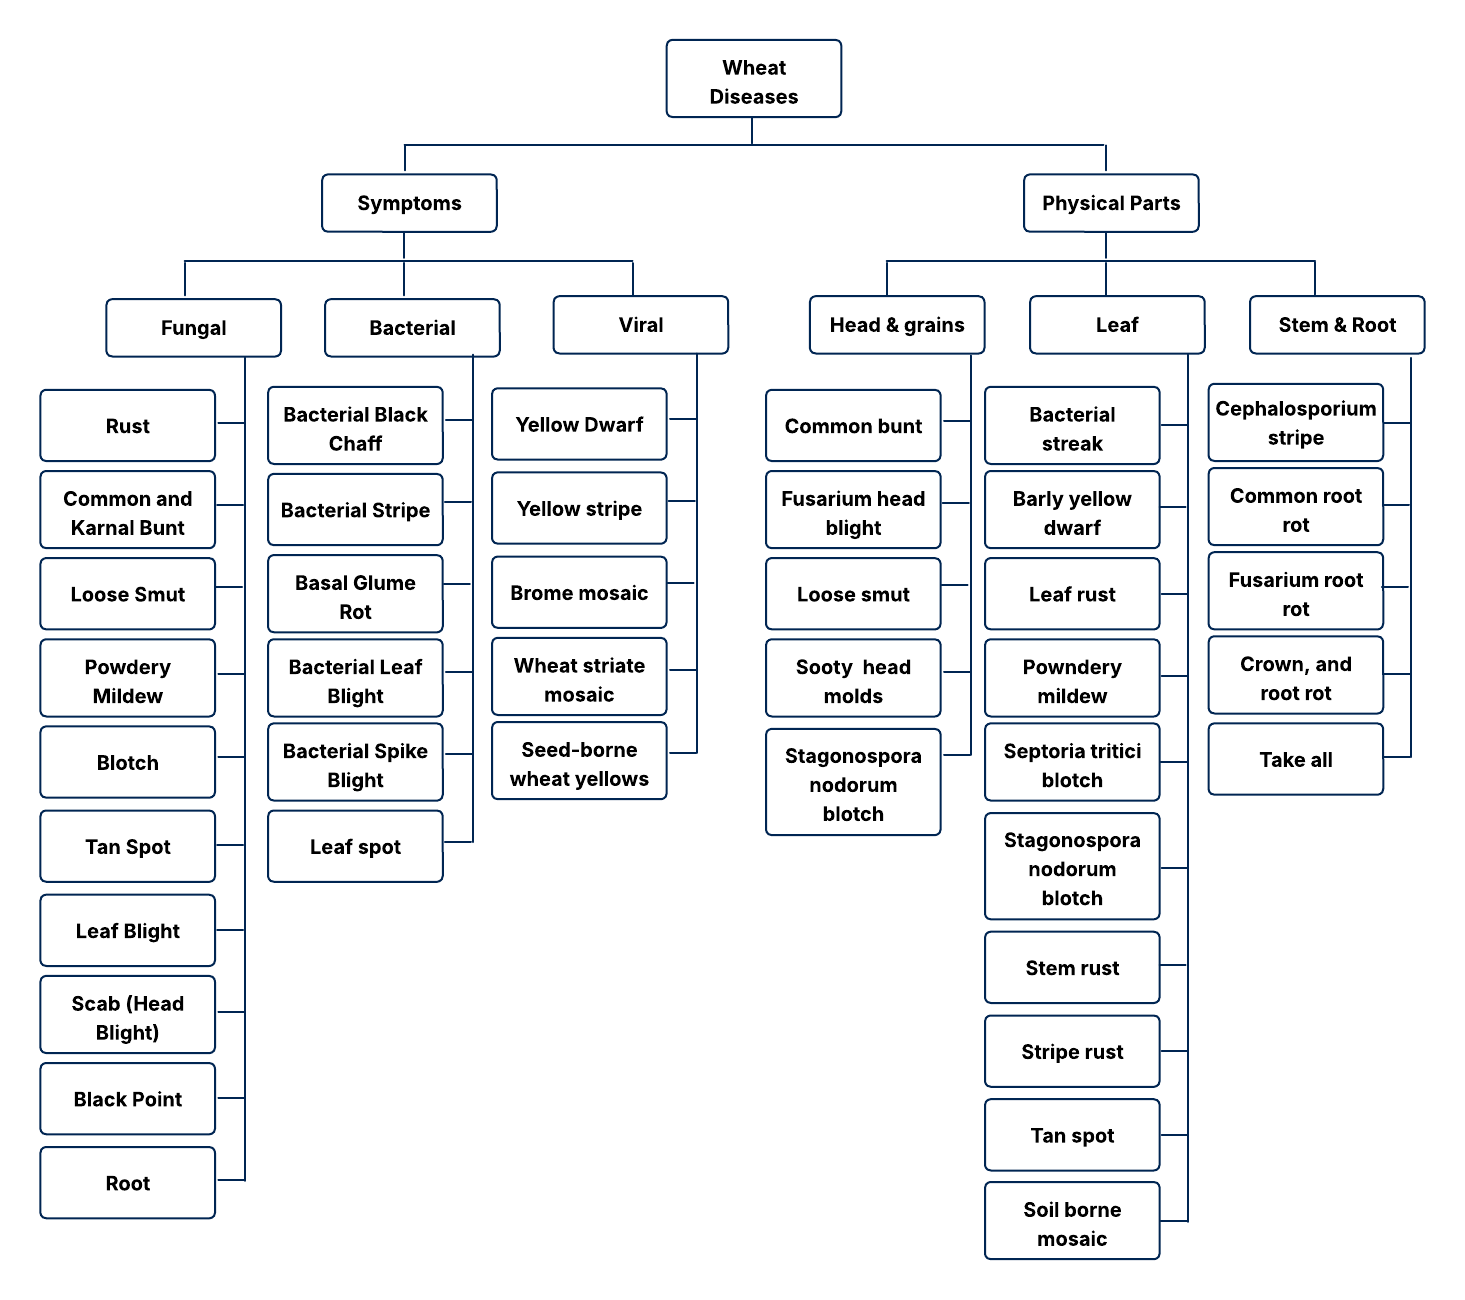
\includegraphics[width=1
    \textwidth]{chapters/chapter2/images/Figure02.png}
    \caption{Taxonomy of wheat diseases \protect\parencite{haider2021wheat}}
    \label{fig:Figure02}
\end{figure}


\begin{itemize}
    \item \textbf{Leaf rust (Brown rust):} Caused by \textit{Puccinia triticina}, it appears as small orange-brown pustules on the upper surfaces of leaves. It spreads quickly in moist environments (~20°C), and advanced stages show black spores. Severe infections reduce grain yield and quality \parencite{duveiller2012wheat}.

    \item \textbf{Stem rust (Black rust):} Caused by \textit{Puccinia graminis}, it produces dark reddish-brown pustules on stems and leaves. Pustules may merge and feel rough. It spreads via wind-borne spores and can cause major crop losses \parencite{duveiller2012wheat}.

    \item \textbf{Stripe rust (Yellow rust):} Caused by \textit{Puccinia striiformis}, this disease forms narrow yellow-orange stripes on leaves and glumes. It thrives in moist conditions between 10–20°C and affects yield and grain quality \parencite{duveiller2012wheat}.

    \item \textbf{Blotch diseases:} These include Septoria tritici blotch, Septoria nodorum blotch, and tan spot, caused by \textit{Zymoseptoria tritici}, \textit{Parastagonospora nodorum}, and \textit{Pyrenophora tritici-repentis} respectively. They cause necrotic blotches on foliage \parencite{figueroa2018review}.

    \item \textbf{Fusarium Head Blight (FHB):} Caused by \textit{Fusarium graminearum}, this disease shows dark, oily florets with pinkish spores. It spreads in warm, humid conditions and may cause mycotoxin contamination in grains \parencite{duveiller2012wheat, figueroa2018review}.

    \item \textbf{Loose smut:} Caused by \textit{Ustilago tritici}, it replaces wheat spikes with black spores. The infection stays dormant in seeds and becomes active during flowering \parencite{duveiller2012wheat}.

    \item \textbf{Powdery mildew:} Caused by \textit{Blumeria graminis f. sp. tritici}, it appears as white powdery spots on leaves. It thrives in cool, dry climates and may reduce yield by up to 40\% \parencite{singh2023wheat}.

    \item \textbf{Common root rot:} Caused by \textit{Cochliobolus sativus}, \textit{Fusarium spp.}, and \textit{Pythium spp.}, it darkens and weakens roots and crowns, reducing plant growth and yield \parencite{duveiller2012wheat}.
\end{itemize}

% \begin{figure}[H]
%     \centering

%     \subfloat[]{\fbox{
%         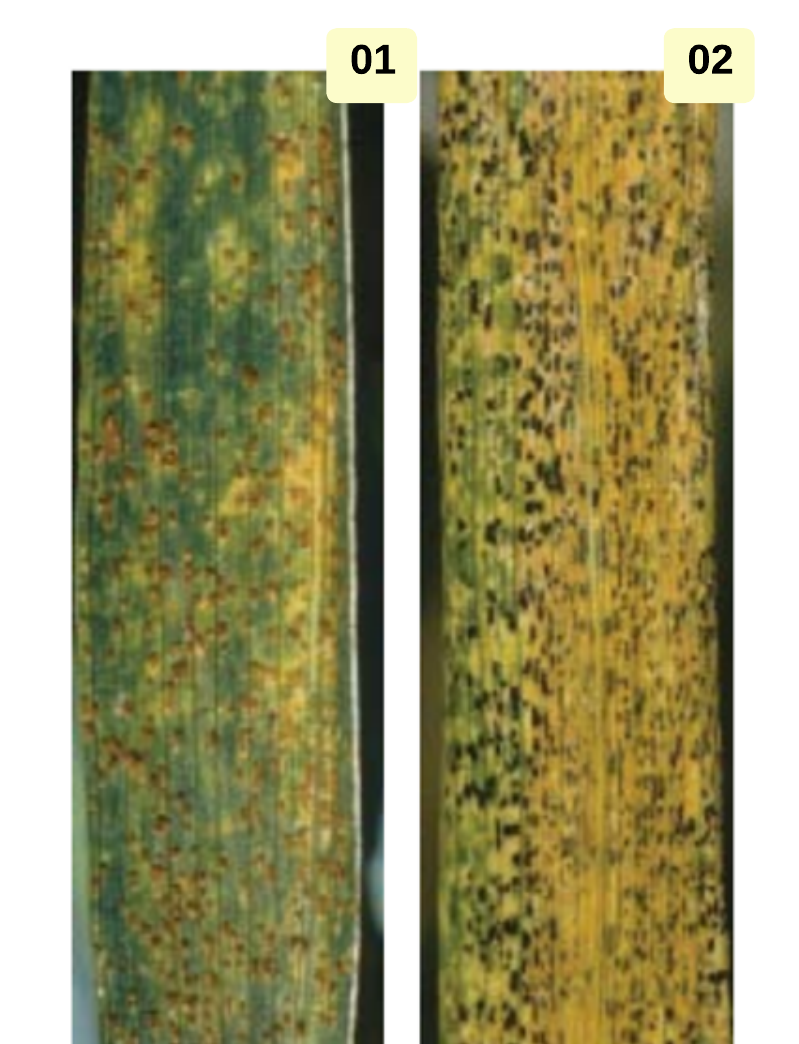
\includegraphics[width=5cm,height=4cm,keepaspectratio]{chapters/chapter2/images/Figure21.png}
%     }}
%     \subfloat[]{\fbox{
%         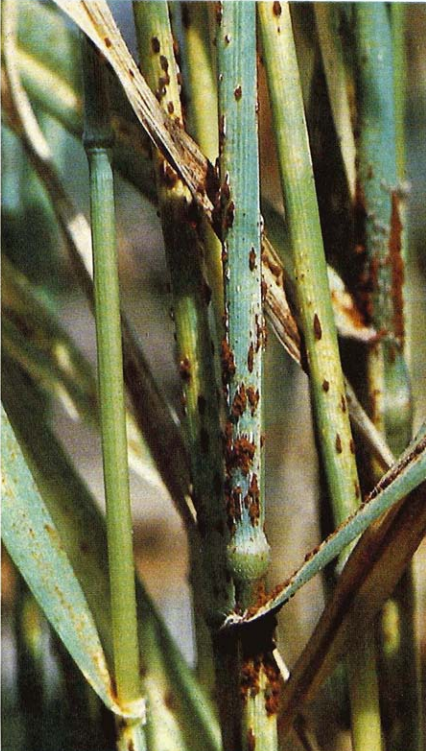
\includegraphics[width=5cm,height=4cm,keepaspectratio]{chapters/chapter2/images/Figure04.png}
%     }}
%     \subfloat[]{\fbox{
%         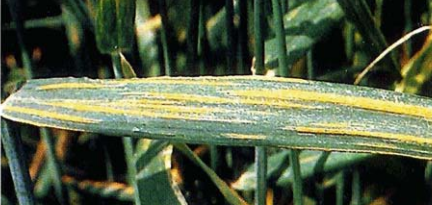
\includegraphics[width=5cm,height=4cm,keepaspectratio]{chapters/chapter2/images/Figure05.png}
%     }}\\[-0.2em]

%     \subfloat[]{\fbox{
%         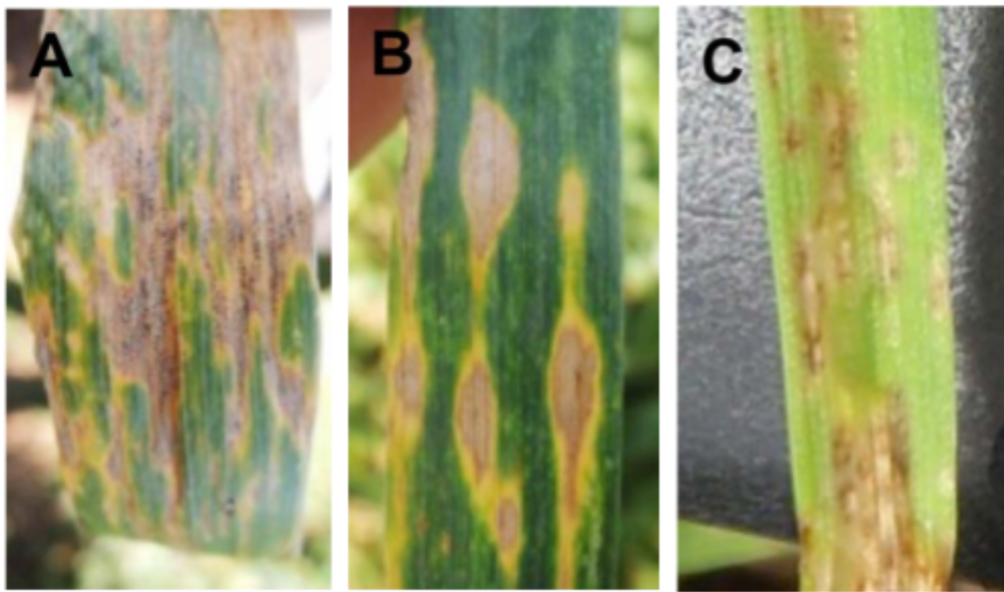
\includegraphics[width=5cm,height=4cm,keepaspectratio]{chapters/chapter2/images/Figure06.png}
%     }}
%     \subfloat[]{\fbox{
%         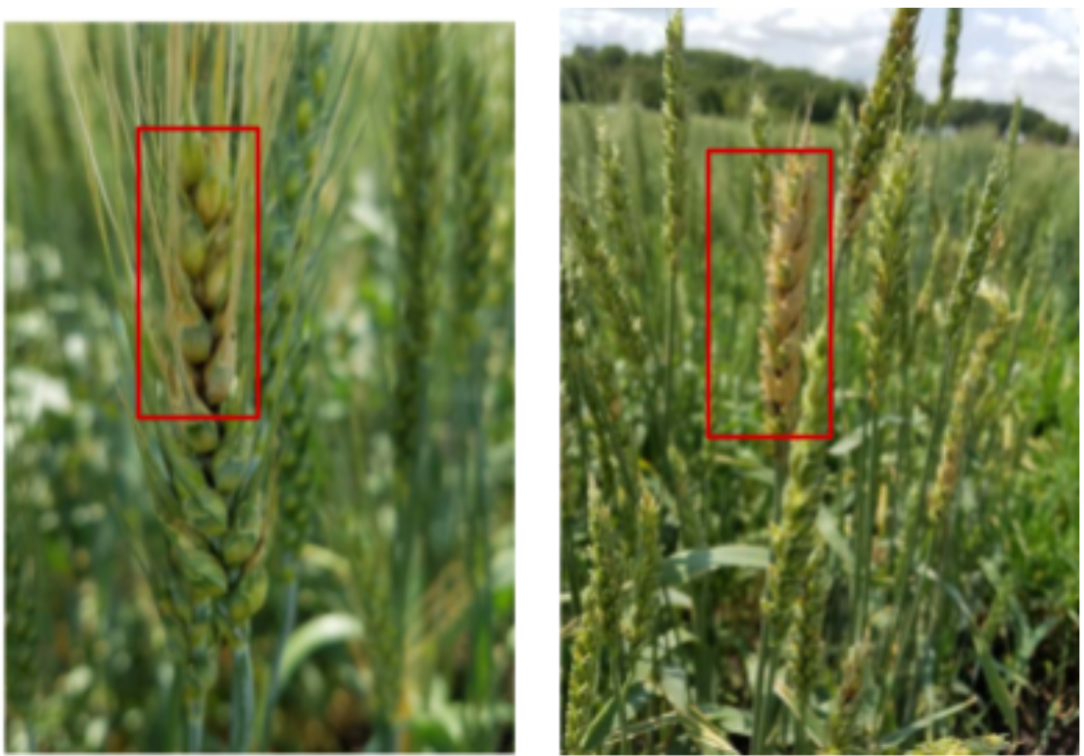
\includegraphics[width=5cm,height=4cm,keepaspectratio]{chapters/chapter2/images/Figure07.png}
%     }}
%     \subfloat[]{\fbox{
%         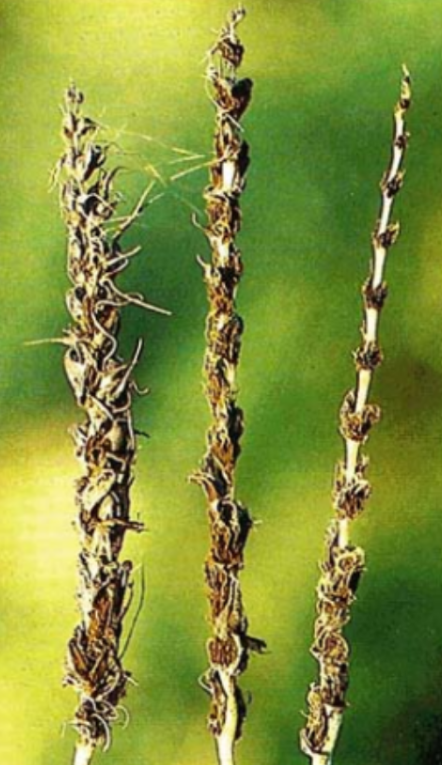
\includegraphics[width=5cm,height=4cm,keepaspectratio]{chapters/chapter2/images/Figure20.png}
%     }}\\[-0.2em]

%     \subfloat[]{\fbox{
%         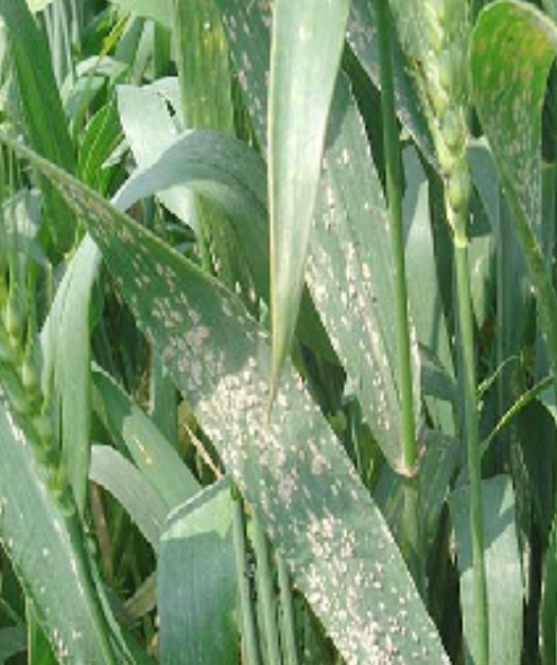
\includegraphics[width=5cm,height=4cm,keepaspectratio]{chapters/chapter2/images/test.png}
%     }}
%     \subfloat[]{\fbox{
%         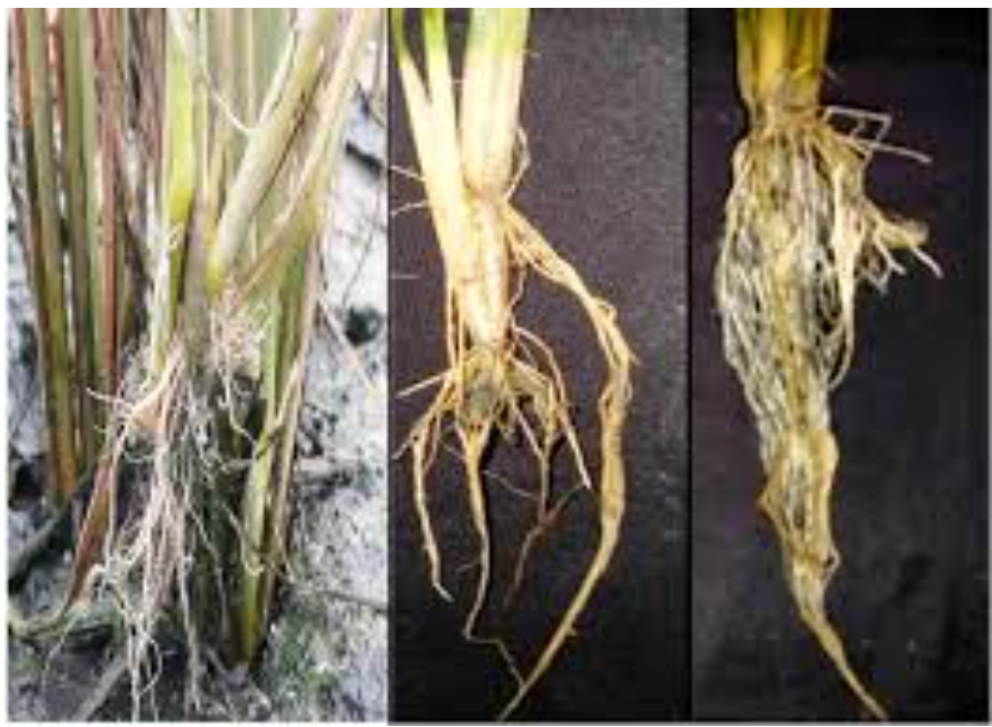
\includegraphics[width=5cm,height=4cm,keepaspectratio]{chapters/chapter2/images/Figure10.png}
%     }}

%     \caption{
%         Common fungal diseases affecting wheat crops:
%         (a) Leaf rust \protect\parencite{duveiller2012wheat},
%         (b) Stem rust \protect\parencite{duveiller2012wheat},
%         (c) Stripe rust \protect\parencite{duveiller2012wheat},
%         (d) Blotch diseases \protect\parencite{figueroa2018review},
%         (e) Fusarium Head Blight \protect\parencite{figueroa2018review},
%         (f) Loose smut \protect\parencite{duveiller2012wheat},
%         (g) Powdery mildew \protect\parencite{singh2023wheat},
%         (h) Common root rot \protect\parencite{duveiller2012wheat}.
%     }
%     \label{fig:wheat-diseases}
% \end{figure}




\begin{figure}[H]
    \centering
    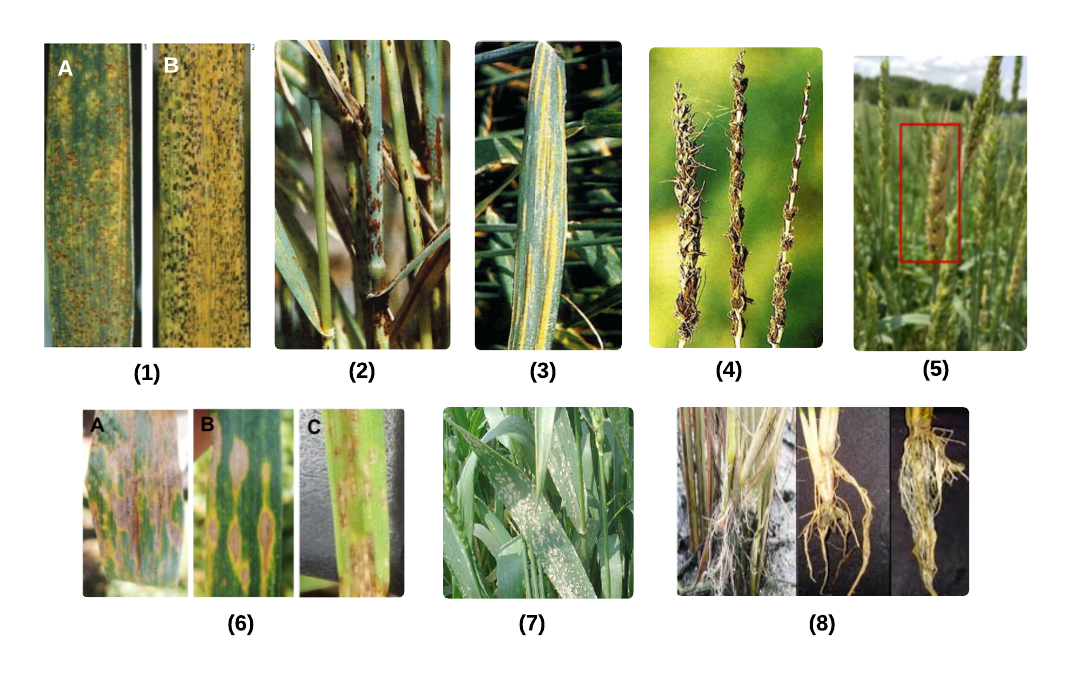
\includegraphics[width=1
    \textwidth]{chapters/chapter13/images/WheatDiseases.png}
    \caption{
        Common fungal diseases affecting wheat crops:
        (1) Leaf rust with Brown spores (A), Leaf rust with Black spores (B) \protect\parencite{duveiller2012wheat},
        (2) Stem rust \protect\parencite{duveiller2012wheat},
        (3) Stripe rust \protect\parencite{duveiller2012wheat},
        (4) Loose smut \protect\parencite{duveiller2012wheat},
        (5) Fusarium Head Blight \protect\parencite{figueroa2018review},
        (6) Symptoms of foliar blotch diseases. (A) Septoria tritici blotch. (B) Tan spot. (C) Septoria nodorum blotch \protect\parencite{figueroa2018review},
        (7) Powdery mildew \protect\parencite{singh2023wheat},
        (8) Common root rot \protect\parencite{duveiller2012wheat}.
    }
    \label{fig:wheat-diseases}
\end{figure}


\section{Common insect pests in wheat cultivation}
Wheat is affected by several insect pests that can seriously reduce yield and quality. Below are some of the most common pests and their impacts (see \autoref{fig:wheat-pests}).
\begin{itemize}
    \item \textbf{Aphids:} Aphids are soft-bodied, transparent insects that feed on wheat leaves and grain heads, causing yellowing, leaf rolling, and poor pollination, especially during early growth. Their sap-sucking damages crops, and the honeydew they excrete promotes black sooty mold, reducing photosynthesis and leading to yield losses of 20–80\% \parencite{duveiller2012wheat,farook2019insect}.

    \item \textbf{Cereal leaf beetle:} Adult cereal leaf beetles are 4–5 mm long with a black head, light brown thorax, and shiny blue-green wings. Larvae are initially yellow but turn into a black mass due to accumulated fecal material. The main symptom of infestation is distinct longitudinal stripes on leaves caused by the feeding of both adults and larvae. Infestations can lead to yield losses of 14\% to over 25\% in winter and fall-sown spring wheat \parencite{duveiller2012wheat}.

    \item \textbf{Armyworm:} The armyworm (Mythimna separata) is a wheat pest. Adult moths are stout and pale brown, while larvae have orange, white, and brown stripes, along with black spots on their prolegs. Caterpillars cause significant damage by swarming from field to field, feeding on seedling leaves and ear heads, which halts plant growth \parencite{farook2019insect}.

    \item \textbf{Brown wheat mite:} The brown wheat mite, found in rainfed wheat areas, has only females that lay red eggs in winter and white-covered eggs in summer. They damage crops by sucking sap, causing silvery flecks, yellowing leaves, and reduced grain quality. Mites are active in daylight and do not form webs. Infestations start in December–January and last until maturity, with winter rains limiting their spread \parencite{kashyap2018identification}.

    \item \textbf{Pink stem borer:} The pink stem borer (Sesamia inferens) is an oriental pest that originally affected rice but has adapted to wheat in North-Western India. Its larvae feed inside wheat stems, causing "dead hearts" and "white heads," leading to yield losses over 11\%. Damage symptoms in wheat are similar to those in rice \parencite{farook2019insect}.

    \item \textbf{Sawfly:} Sawflies produce one generation per year, with larvae overwintering in straw. The legless white larvae bore into wheat stems, weakening plants, causing poor head development, and making them prone to lodging. While infestations are patchy, the wheat stem sawfly (Cephus cinctus) can cause severe localized yield losses \parencite{duveiller2012wheat}.

    \item \textbf{Slugs, Snails, Grasshoppers, and Crickets:} These are widespread pests affecting wheat and other plants. They damage crops by chewing leaves, causing a frayed appearance in mature plants. While their presence is often localized, large infestations can significantly impact plant health and yield worldwide.

    \item \textbf{Wireworm:} Wireworms are yellow to brown larvae with six short legs that feed on wheat kernels, consuming the endosperm and leaving only the seed coat. They attack young seedlings, causing "damping off" symptoms and damaging crops early on. Their presence can significantly affect wheat growth and yield, making timely identification and control crucial \parencite{farook2019insect}.
\end{itemize}

\begin{figure}[H]
    \centering
    \subfloat[Aphids \protect\parencite{farook2019insect}]{
        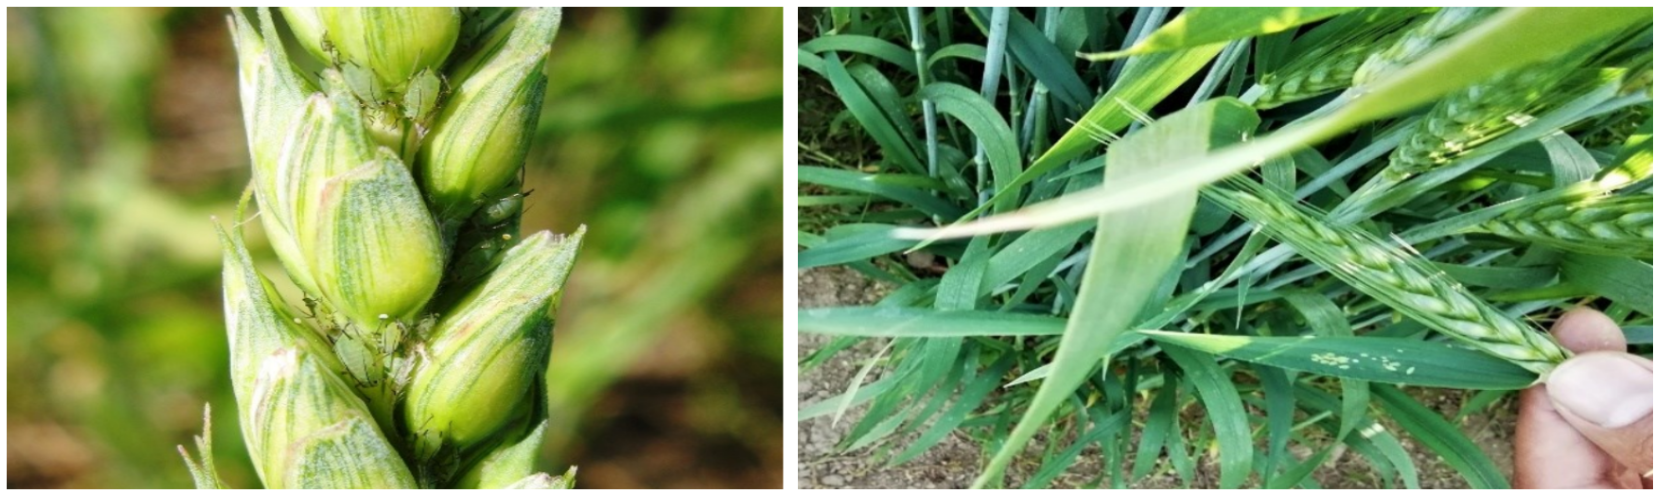
\includegraphics[width=0.3\textwidth,height=0.17\textwidth]{chapters/chapter2/images/Figure11.png}
    }
    \subfloat[Cereal leaf beetle \protect\parencite{farook2019insect}]{
        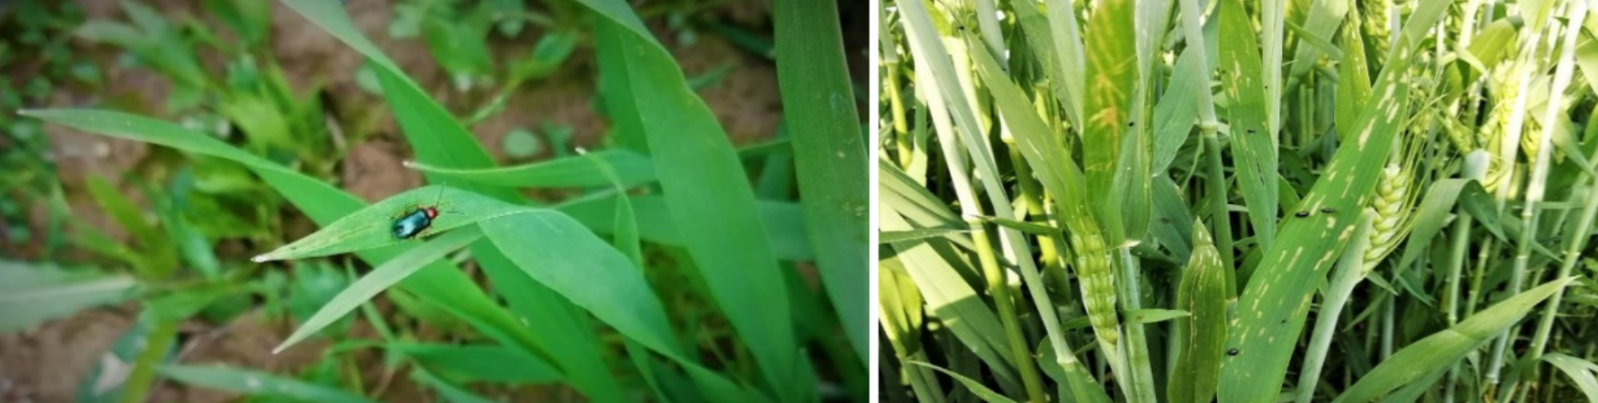
\includegraphics[width=0.3\textwidth,height=0.17\textwidth]{chapters/chapter2/images/Figure12.png}
    }
    \subfloat[Armyworm \protect\parencite{farook2019insect}]{
        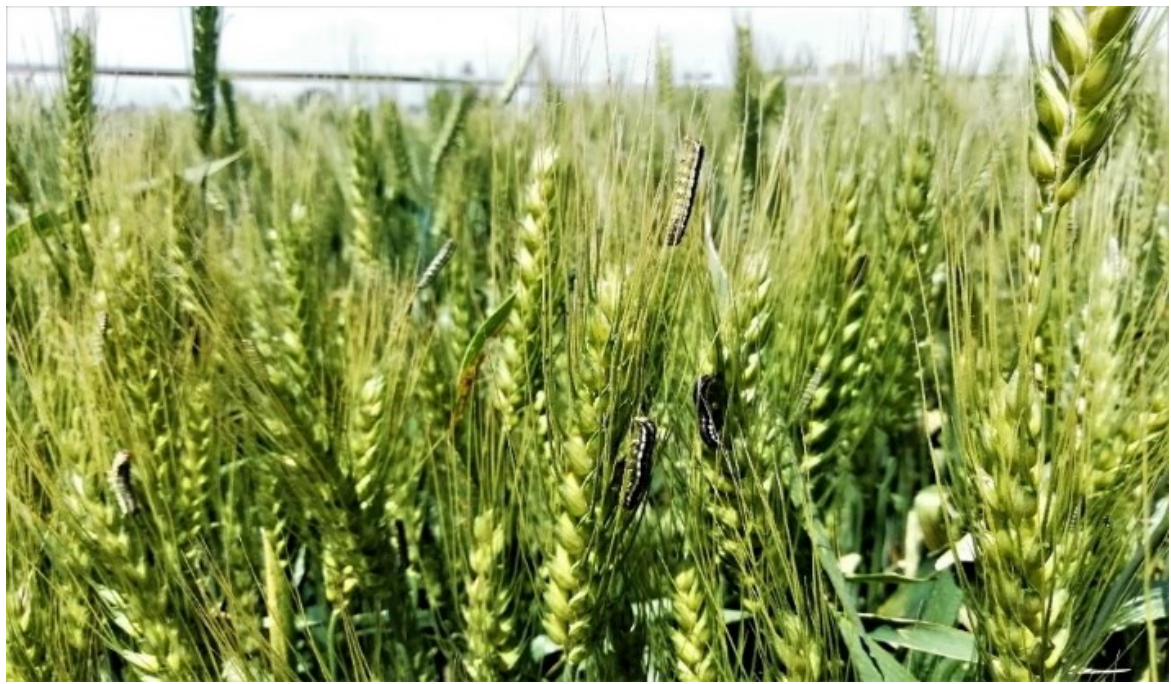
\includegraphics[width=0.3\textwidth,height=0.17\textwidth]{chapters/chapter2/images/Figure13.png}
    }\\[-0.2em]

    \subfloat[Brown wheat mite \protect\parencite{kashyap2018identification}]{
        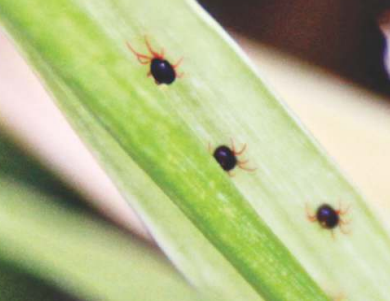
\includegraphics[width=0.3\textwidth,height=0.17\textwidth]{chapters/chapter2/images/Figure15.png}
    }
    \subfloat[Pink stem borer \protect\parencite{farook2019insect}]{
        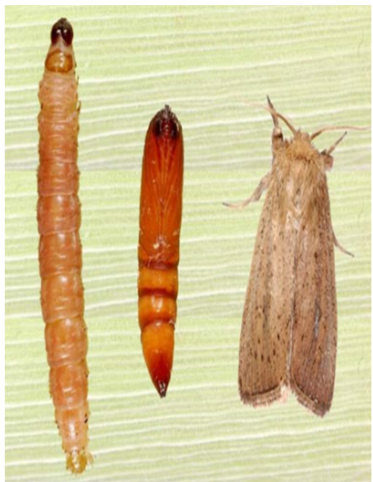
\includegraphics[width=0.3\textwidth,height=0.17\textwidth]{chapters/chapter2/images/Figure16.png}
    }
    \subfloat[Sawfly (Kaggle "Dataset IP102")]{
        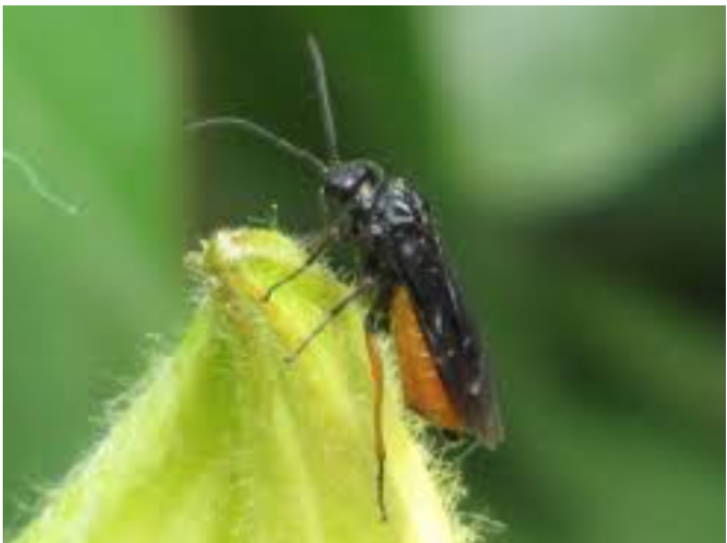
\includegraphics[width=0.3\textwidth,height=0.17\textwidth]{chapters/chapter2/images/Figure17.png}
    }\\[-0.2em]

    \subfloat[Grasshoppers (Kaggle "Dataset IP102")]{
        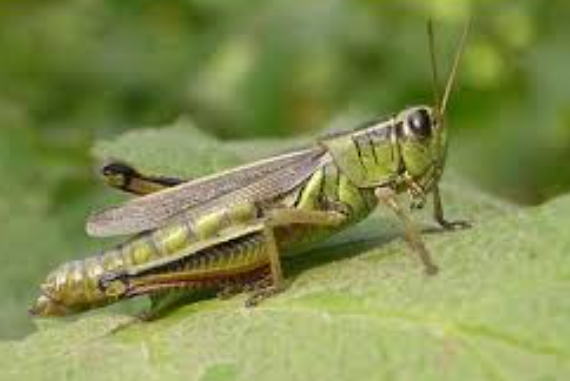
\includegraphics[width=0.3\textwidth,height=0.17\textwidth]{chapters/chapter2/images/Figure18.png}
    }
    \subfloat[Wireworm \protect\parencite{farook2019insect}]{
        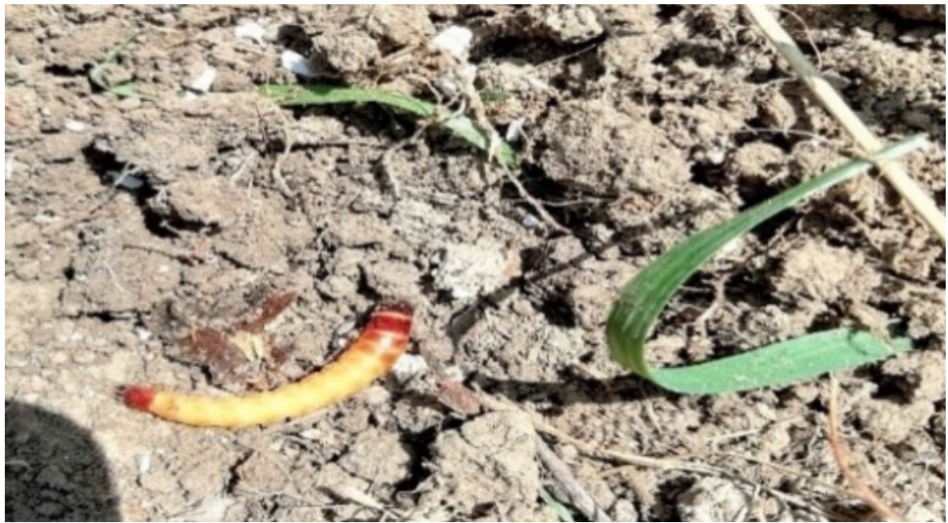
\includegraphics[width=0.3\textwidth,height=0.17\textwidth]{chapters/chapter2/images/Figure19.png}
    }

    \caption{Common pests affecting wheat crops.}
    \label{fig:wheat-pests}
\end{figure}


\section{Enhancing wheat disease control strategies}

Effective wheat disease management combines traditional farming practices with modern technologies. Together, they offer a balanced approach to reducing disease impact and improving crop health.

\subsection*{Usual instruments (Classic methods)}
Traditional methods are widely used to manage wheat diseases and improve crop health. These include crop rotation to break disease cycles, proper tillage to manage soil pathogens, and using clean seeds to avoid spreading infections. Maintaining healthy soil and applying balanced fertilizers help plants grow stronger and resist diseases. Choosing resistant wheat varieties, changing sowing dates, and using eco-friendly practices like field cleaning and proper spacing also reduce the chances of disease spreading \parencite{mehta2014wheat}.

\subsection*{Technological tools}
Complementing traditional methods, the following tools, rooted in smart agriculture, offer modern solutions to enhance the effectiveness and precision of wheat disease management.

\begin{itemize}
    \item \textbf{Remote sensing:} Remote sensing using unmanned aerial vehicle-mounted multispectral sensors enables high-resolution monitoring of wheat canopy characteristics across different growth stages. By analyzing spectral bands (Green, Red, Red Edge, Near Infrared), the system captures critical indicators of plant health, canopy structure, and stress conditions, supporting precise and timely crop management \parencite{zhang2025precision}.
    \item \textbf{Disease forecast modeling:} Weather-based and biological models are used to predict disease outbreaks and support timely interventions \parencite{mehta2014wheat}.
    \item \textbf{Computer vision:} Enables automated analysis of crop images for monitoring wheat growth, detecting diseases, and assessing yield. It plays a crucial role in real-time decision-making by processing visual data from the field \parencite{ghazal2024computer}.
    \item \textbf{\gls{abb:ai} and \gls{abb:ml} algorithms:} Used to interpret complex image data, these algorithms support tasks like disease classification, crop health prediction, and optimizing farm operations by learning from patterns in large agricultural datasets \parencite{ghazal2024computer}.
    \item \textbf{Autonomous robotic platforms and drones:} Facilitate efficient field data collection, spraying, and crop monitoring. These tools reduce manual labor and enable precise, targeted interventions across large wheat fields \parencite{ghazal2024computer}.
    \item \textbf{Precision agriculture systems:} Precision agriculture systems integrate technologies like the \gls{abb:gps} and the \gls{abb:iot} to manage field variability. These technologies help optimize the use of inputs (e.g., water, fertilizer) and support sustainable, data-driven wheat farming. \parencite{ghazal2024computer}.
\end{itemize}


\section{Challenges facing the integration of smart agricultural systems}
Fully automated smart farming faces both technical and practical challenges. A major obstacle is the generalization of computer vision models across diverse field conditions like lighting, weather, soil, and crop types, which complicates real-time deployment. Robust decision-making in unpredictable outdoor environments also remains difficult, and integrating the full pipeline from image capture to treatment is still under development \parencite{ghazal2024computer}.

On the technical side, communication protocols often support only short distances, limiting scalability. Many devices rely on batteries, reducing operational time. Additionally, processing the large volumes of data generated introduces computational bottlenecks, alongside concerns about privacy, trust, and security in data handling \parencite{idoje2021survey}.



\section{Review of Image-Based Approaches in Wheat Disease Identification}

In recent years, image-based approaches leveraging advances in deep learning have emerged as powerful tools for wheat diseases classification. These methods rely on the visual symptoms present on wheat leaves, stems, or spikes, captured through images and analyzed using automated algorithms.



\subsection{Approaches in data collection and preprocessing }
This section discusses various methods employed in the literature for gathering data, handling challenges such as low-quality or irrelevant images, and preprocessing techniques that prepare datasets for effective utilization in classification and detection tasks.

\subsubsection{Data collection}
The initial and foundational step in developing deep learning models for wheat disease classification is the acquisition of high-quality and diverse image data. This data can be sourced through various means, including manual and automated methods. Common sources include drone-mounted or mobile device cameras, which allow for the real-time capture of wheat leaf images under natural field conditions. Public datasets also play a crucial role; for instance, the "Wheat Leaf Dataset" available on Kaggle, utilized by \parencite{ramadan2024improving}, and the "Wheat Disease Detection" dataset, employed by \parencite{reis2024integrated}, offer extensive repositories of labeled images. In addition to these, hybrid data collection strategies are often employed. \parencite{hassan2024wheat}, for example, combined images obtained from field visits, Kaggle datasets, and internet sources to enrich their training data. This diversity in data sources helps improve the robustness and generalization capability of the resulting models.


\subsubsection{Data preprocessing}
Data preprocessing plays an important role in improving the quality and relevance of input images for deep learning models. This process typically begins with the elimination of low-quality images where disease symptoms are poorly visible \parencite{yao2024yolo} and the cropping of extraneous image regions to concentrate on areas of diagnostic interest. To further enhance the visual quality, advanced contrast enhancement techniques such as Contrast Limited Adaptive Histogram Equalization (CLAHE), contrast stretching, and the hypercolumn technique (Figure~\ref{fig:CLAHE}) are commonly employed to improve image contrast and brightness, as discussed by \parencite{reis2024integrated} and \parencite{fang2023lightweight}. These methods significantly improve image contrast and brightness, making subtle disease features more discernible and thereby facilitating more accurate classification. Additionally, to isolate the region of interest and reduce background noise, methods such as background removal, color thresholding, and edge detection are utilized \parencite{alharbi2023wheat}, ensuring that only the most relevant image features are presented to the model.


\begin{figure}[H] % 'H' needs \usepackage{float}
    \centering
    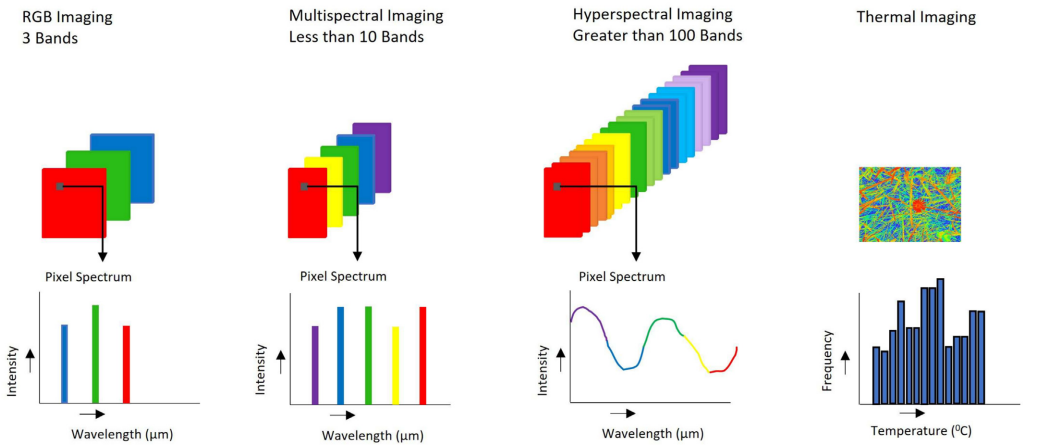
\includegraphics[width=0.8\textwidth]{chapters/chapter3/images/Figure01.png}
    \caption{Sub-data samples of the wheat disease original dataset obtained by the CLAHE, Contrast stretching, and hypercolumn technique \parencite{reis2024integrated}.}
    \label{fig:CLAHE}
\end{figure}

\subsubsection{Data augmentation}

Data augmentation is extensively employed to mitigate class imbalance and enhance dataset diversity, thereby improving the generalization capabilities of deep learning models. Common augmentation techniques include random rotations, cropping, zooming, flipping, and contrast adjustments (Figure~\ref{fig:Dataaugmentation}), which artificially expand the training dataset by introducing varied visual representations of the original images \parencite{nagpal2024hybrid,hassan2024wheat,nigam2023deep}.

\begin{figure}[H] % 'H' needs \usepackage{float}
    \centering
    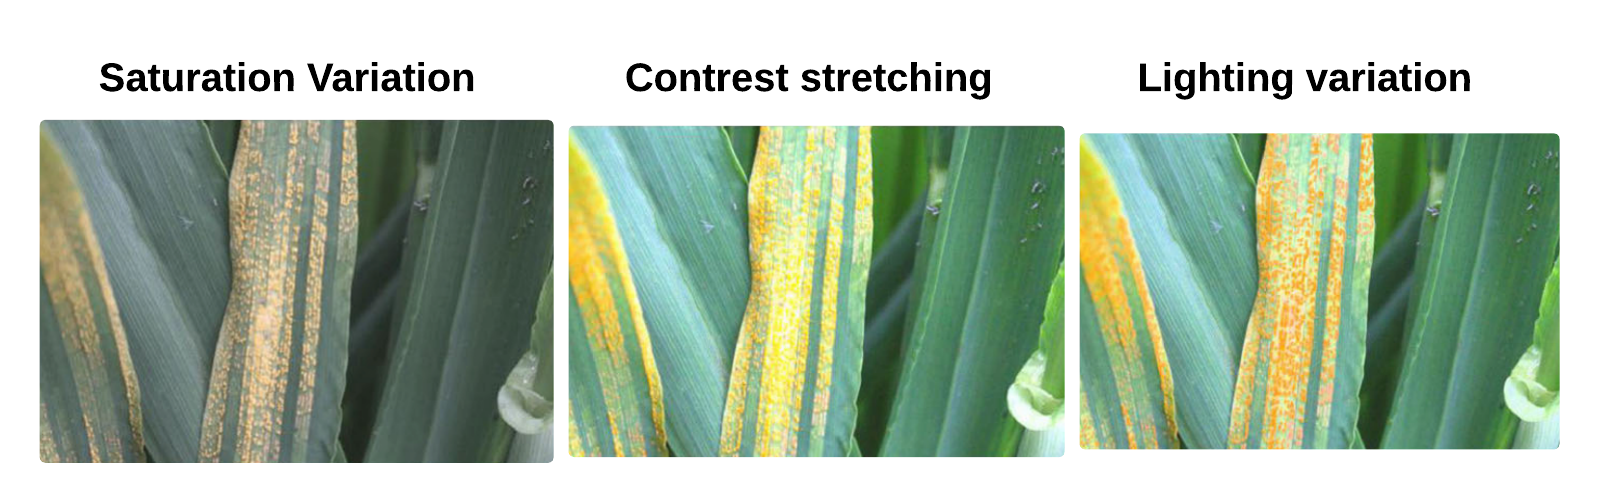
\includegraphics[width=0.8\textwidth]{chapters/chapter3/images/Figure02.png}
    \caption{Data augmentation techniques \parencite{nagpal2024hybrid}.}
    \label{fig:Dataaugmentation}
\end{figure}

\parencite{ramadan2024improving} use four augmentation techniques enhance dataset diversity and address class imbalance: CycleGAN, which generates realistic synthetic images through unpaired image-to-image translation; ADASYN, which adaptively oversamples difficult minority class instances; SMOTE, which creates synthetic samples by interpolating between minority class neighbors; and SMOTE-Tomek, a hybrid method that combines SMOTE with Tomek links to both oversample and remove noisy boundary samples.



\subsection{Approaches in wheat disease classification}

Various classification models have been employed in the literature to address wheat disease classification effectively. These approaches, preprocessing techniques, datasets, classification categories, and results are summarized in Table~\ref{tab:wheat-disease-related-work}, which provides a comparative overview of the most recent and relevant studies in this domain.




\begin{longtable}{|p{3cm}|p{6cm}|p{3.5cm}|p{2.5cm}|}
\caption{Related work on wheat disease classification} \label{tab:wheat-disease-related-work} \\
\hline
\textbf{Reference} & \textbf{Method and Preprocessing} & \textbf{Categories and Dataset} & \textbf{Results} \\
\hline
\endfirsthead
\endhead

\parencite{ramadan2024improving} & 
\begin{itemize}
    \item \textbf{Method:} Pre-trained \gls{abb:cnn}s (DenseNet121, ResNet50V2, MobileNetV2, Xception)
    \item \textbf{Preprocessing:} CycleGAN, ADASYN, SMOTE, SMOTETomek
\end{itemize} &
\begin{itemize}
    \item \textbf{Categories:} Healthy, stripe rust, septoria
    \item \textbf{Dataset:} Wheat Leaf Dataset (407 images)
\end{itemize} &
CycleGAN + MobileNetV2: 100\% accuracy \\
\hline

\parencite{nagpal2024hybrid} & 
\begin{itemize}
    \item \textbf{Method:} Hybrid (MobileNet + DenseNet + PSO + \gls{abb:svm}/DT/RF)
    \item \textbf{Preprocessing:} Resize, normalize, augment (flip, rotate, crop, noise, zoom)
\end{itemize} &
\begin{itemize}
    \item \textbf{Categories:} Yellow rust, brown rust, loose smut, healthy
    \item \textbf{Dataset:} Custom (887 images)
\end{itemize} &
98.89\% \\
\hline

\parencite{reis2024integrated} &
\begin{itemize}
    \item \textbf{Method:} Deep models + Ensemble learning
    \item \textbf{Preprocessing:} CLAHE, hypercolumn
\end{itemize} &
\begin{itemize}
    \item \textbf{Categories:} Healthy, yellow rust, brown rust
    \item \textbf{Dataset:} Wheat Disease Detection Dataset (2400 images)
\end{itemize} &
99.72\% \\
\hline

\parencite{goyal2021leaf} &
\begin{itemize}
    \item \textbf{Method:} Deep \gls{abb:cnn}
    \item \textbf{Preprocessing:} /
\end{itemize} &
\begin{itemize}
    \item \textbf{Categories:} 10 (karnal bunt, powdery mildew, etc.)
    \item \textbf{Dataset:} LWDCD2020 (12,000 images)
\end{itemize} &
97.88\% \\
\hline

\parencite{alharbi2023wheat} &
\begin{itemize}
    \item \textbf{Method:} Few-shot learning + EfficientNet + attention
    \item \textbf{Preprocessing:} /
\end{itemize} &
\begin{itemize}
    \item \textbf{Categories:} 18 classes
    \item \textbf{Dataset:} PlantVillage, CGIAR, manual, Google Images (1530 images)
\end{itemize} &
93.19\% \\
\hline

\parencite{jouini2024wheat} &
\begin{itemize}
    \item \textbf{Method:} CropNet (EfficientNetB0 + shallow \gls{abb:cnn})
    \item \textbf{Preprocessing:} Resize, normalize
\end{itemize} &
\begin{itemize}
    \item \textbf{Categories:} Healthy, septoria, mildew, rusts
    \item \textbf{Dataset:} /
\end{itemize} &
99.80\% \\
\hline

\parencite{fang2023lightweight} &
\begin{itemize}
    \item \textbf{Method:} Inception-ResNet-CE with CBAM/ECA
    \item \textbf{Preprocessing:} Contrast enhancement, augmentation
\end{itemize} &
\begin{itemize}
    \item \textbf{Categories:} 7 (rusts, smut, powdery, etc.)
    \item \textbf{Dataset:} LWDCD2020, PlantVillage, CGIAR
\end{itemize} &
98.76\% \\
\hline

\parencite{nigam2023deep} &
\begin{itemize}
    \item \textbf{Method:} EfficientNet transfer learning
    \item \textbf{Preprocessing:} Contrast, resize, augment
\end{itemize} &
\begin{itemize}
    \item \textbf{Categories:} Stripe rust, stem rust, leaf rust, healthy
    \item \textbf{Dataset:} WheatRust21 (6556 images)
\end{itemize} &
99.35\% \\
\hline

\parencite{jiang2022evaluation} &
\begin{itemize}
    \item \textbf{Method:} 7 \gls{abb:cnn}s (e.g., VGG-16, ResNet-50)
    \item \textbf{Preprocessing:} Resize, normalization, augmentation
\end{itemize} &
\begin{itemize}
    \item \textbf{Categories:} Healthy, mildew, rusts
    \item \textbf{Dataset:} Field-based Wheat Diseases Images (FWDI) (2643 images)
\end{itemize} &
92.5\% \\
\hline

\end{longtable}



\textbf{Transfer learning approaches \parencite{jiang2022evaluation}:}  compares three \gls{abb:cnn} training strategies for wheat disease identification (Figure~\ref{fig:TrainingStrategies}): training from scratch, fixed feature extraction, and transfer learning with fine-tuning.

\begin{itemize}
  \item \textbf{Training from scratch:} In this approach, the entire \gls{abb:cnn} is trained from the ground up with randomly initialized weights, using only the target dataset, namely the \textit{Field-based Wheat Diseases Images (FWDI)} dataset. While this method allows for complete customization of the model architecture and parameters, it demands a large volume of labeled data and substantial computational resources.

  \item \textbf{Fixed feature extraction:} This strategy involves using a pre-trained \gls{abb:cnn} as a fixed feature extractor. All convolutional layers are frozen to retain the learned representations from a source dataset, and only the final classification layers such as the fully connected, batch normalization, and softmax layers are retrained on the target dataset. Typically, the model is pre-trained on a large-scale dataset, then applied to a target dataset. A similar methodology was adopted by \parencite{nigam2023deep}, who fine-tuned a pre-trained EfficientNet model on their custom WheatRust21 dataset for wheat rust classification, achieving a notable accuracy of 99.35\%.

  \item \textbf{Transfer learning with fine-tuning:} This technique involves partially or fully retraining a pre-trained \gls{abb:cnn} on the target dataset, allowing the model to adapt its learned features to the specific characteristics of the new domain. In most cases, the model is initially trained on a diverse and extensive source dataset such as \textit{PlantVillage}, then fine-tuned using a specific dataset. For instance, \parencite{jiang2022evaluation} employed this approach with InceptionV3, reaching an accuracy of 92.5\% on the \textit{FWDI} dataset. Similarly, \parencite{ramadan2024improving} fine-tuned \gls{abb:cnn}s including DenseNet121, ResNet50V2, MobileNetV2, and Xception for wheat leaf disease classification using both augmented and non-augmented datasets. They achieved 100\% accuracy in predicting three classes (healthy, stripe rust, or septoria), further validating the effectiveness of fine-tuning in this domain. This accuracy was specifically achieved by the MobileNetV2 model when trained on data augmented with both CycleGAN and ADASYN.
\end{itemize}




\begin{figure}[H] 
    \centering
    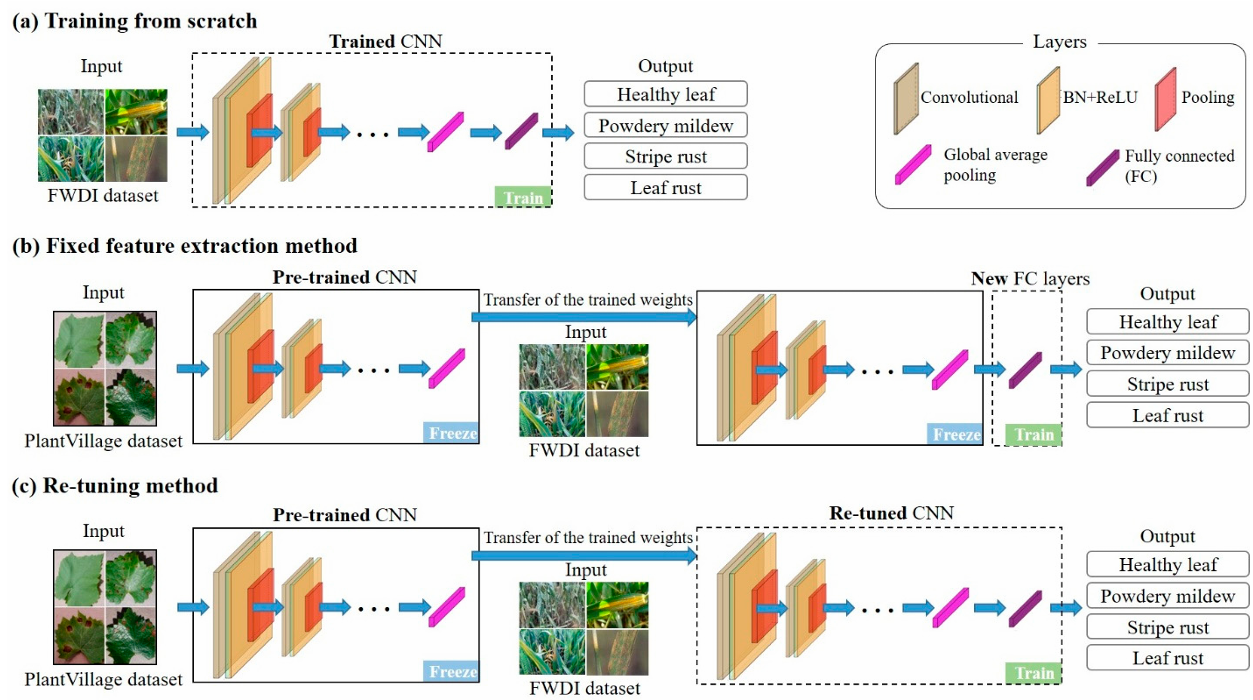
\includegraphics[width=1.1\textwidth]{chapters/chapter3/images/Figure03.png}
    \caption{Training strategies of a convolutional neural network (\gls{abb:cnn}) \parencite{jiang2022evaluation}.}
    \label{fig:TrainingStrategies}
\end{figure}



\textbf{Hybrid models \parencite{nagpal2024hybrid}:} Introduced a hybrid model (Figure~\ref{fig:hybridframework}) that combines deep learning and traditional machine learning for image classification. Features are extracted from images using two pre-trained \gls{abb:cnn} models, MobileNet and DenseNet, and then concatenated. Particle Swarm Optimization (PSO) is applied for dimensionality reduction. Finally, the reduced features are fed into traditional classifiers (\gls{abb:rf}, \gls{abb:svm}, \gls{abb:dt}) for training and prediction, achieving an accuracy of 98.89\% across four classes.


\begin{figure}[H] 
    \centering
    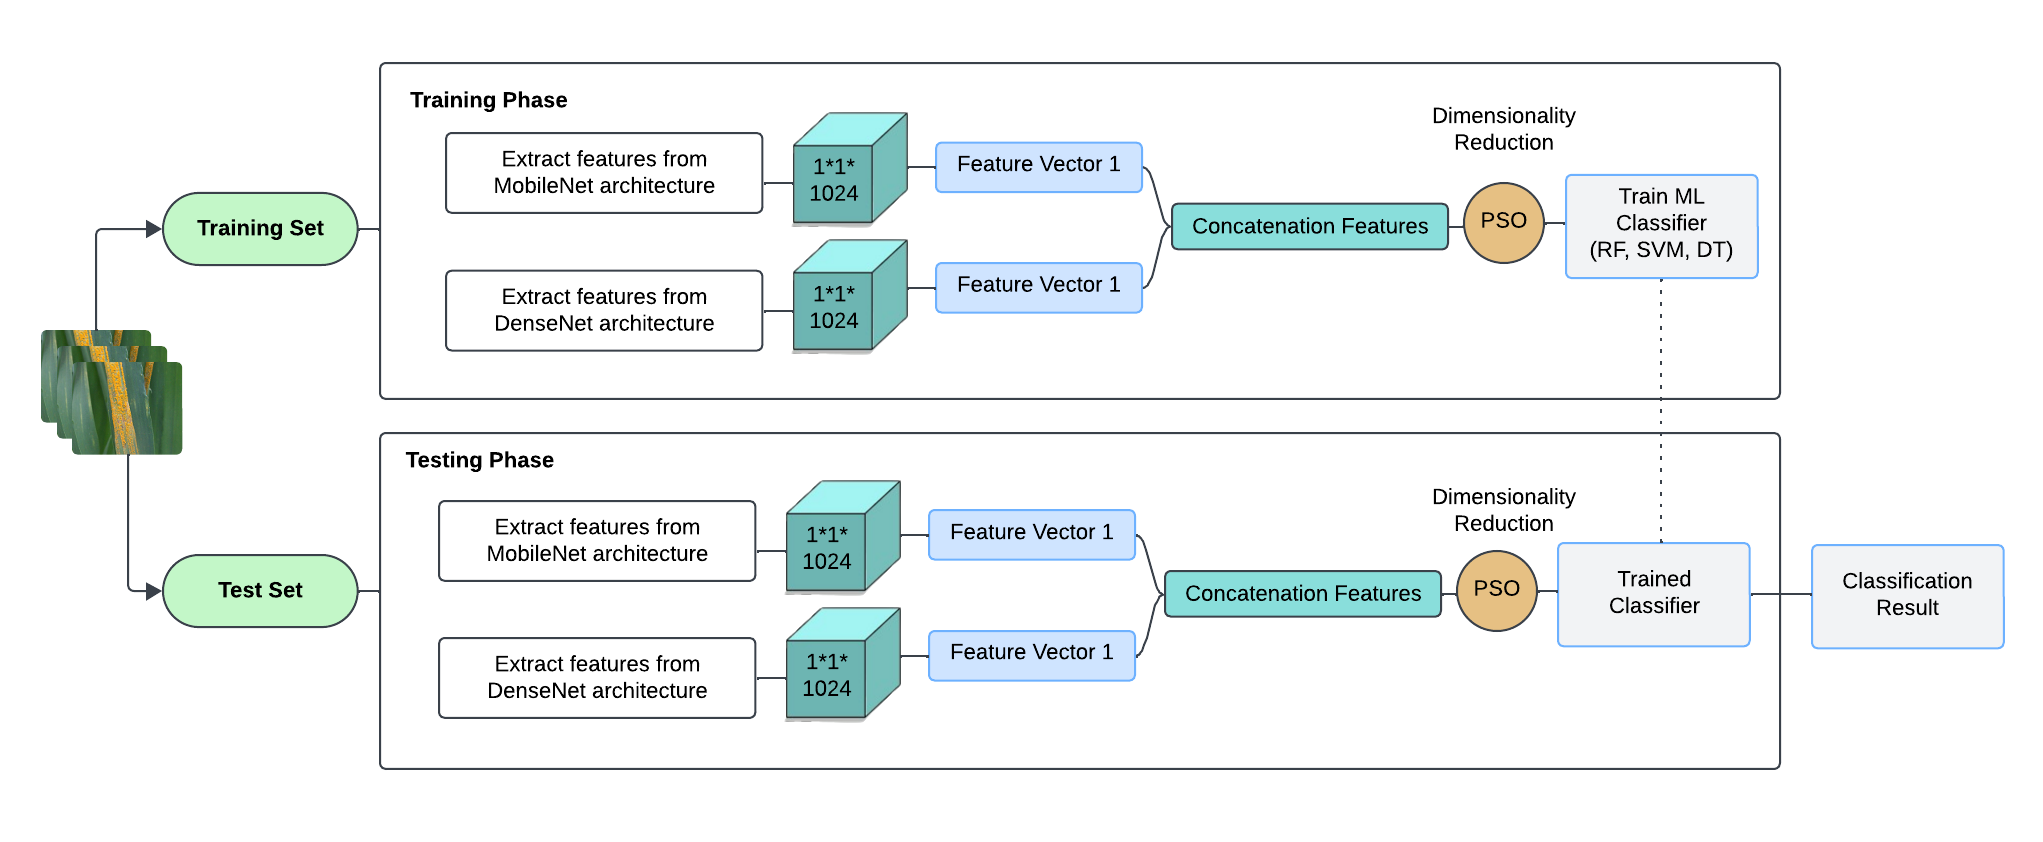
\includegraphics[width=1.1\textwidth]{chapters/chapter3/images/Figure04.png}
    \caption{The architecture of the hybrid framework \parencite{nagpal2024hybrid}.}
    \label{fig:hybridframework}
\end{figure}









\textbf{Custom deep convolutional networks \parencite{goyal2021leaf}:}  Proposed a custom deep convolutional neural network (Figure~\ref{fig:CustomDeepCN}) specifically designed for wheat disease classification. The architecture comprises 21 convolutional layers, 7 max-pooling layers, and 3 fully connected layers. Activation functions used include \gls{abb:relu} and Leaky \gls{abb:relu} in the convolutional layers, while the fully connected layers employ \gls{abb:relu}, followed by a SoftMax classifier for multi-class output. The model was trained on a dataset of over 12,000 labeled RGB images covering 10 distinct wheat disease classes and achieved an accuracy of 97.88\%. 

\begin{figure}[H] 
    \centering
    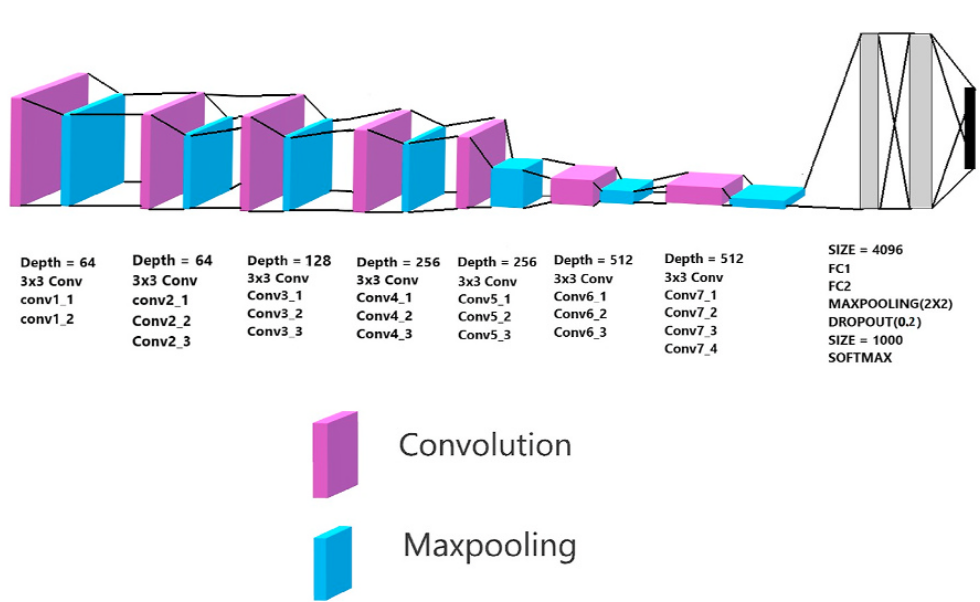
\includegraphics[width=1\textwidth]{chapters/chapter3/images/Figure05.png}
    \caption{The proposed deep convolutional neural network \parencite{goyal2021leaf}.}
    \label{fig:CustomDeepCN}
\end{figure}



\textbf{Few-Shot learning \parencite{alharbi2023wheat}:} This approach uses a Siamese network structure with EfficientNetB0 as a shared feature extractor for both the support set (a few labeled examples) and the query set (unlabeled images to classify). Each image passes through the same feature extractor to generate embeddings. These embeddings are then compared using an attention block, which calculates similarity scores between the query and support images. A softmax function is applied to generate the final similarity-based classification. This model was able to classify 18 wheat disease types with an accuracy of 93.19\% (see figure~\ref{fig:Few-shot}).

\begin{figure}[H] 
    \centering
    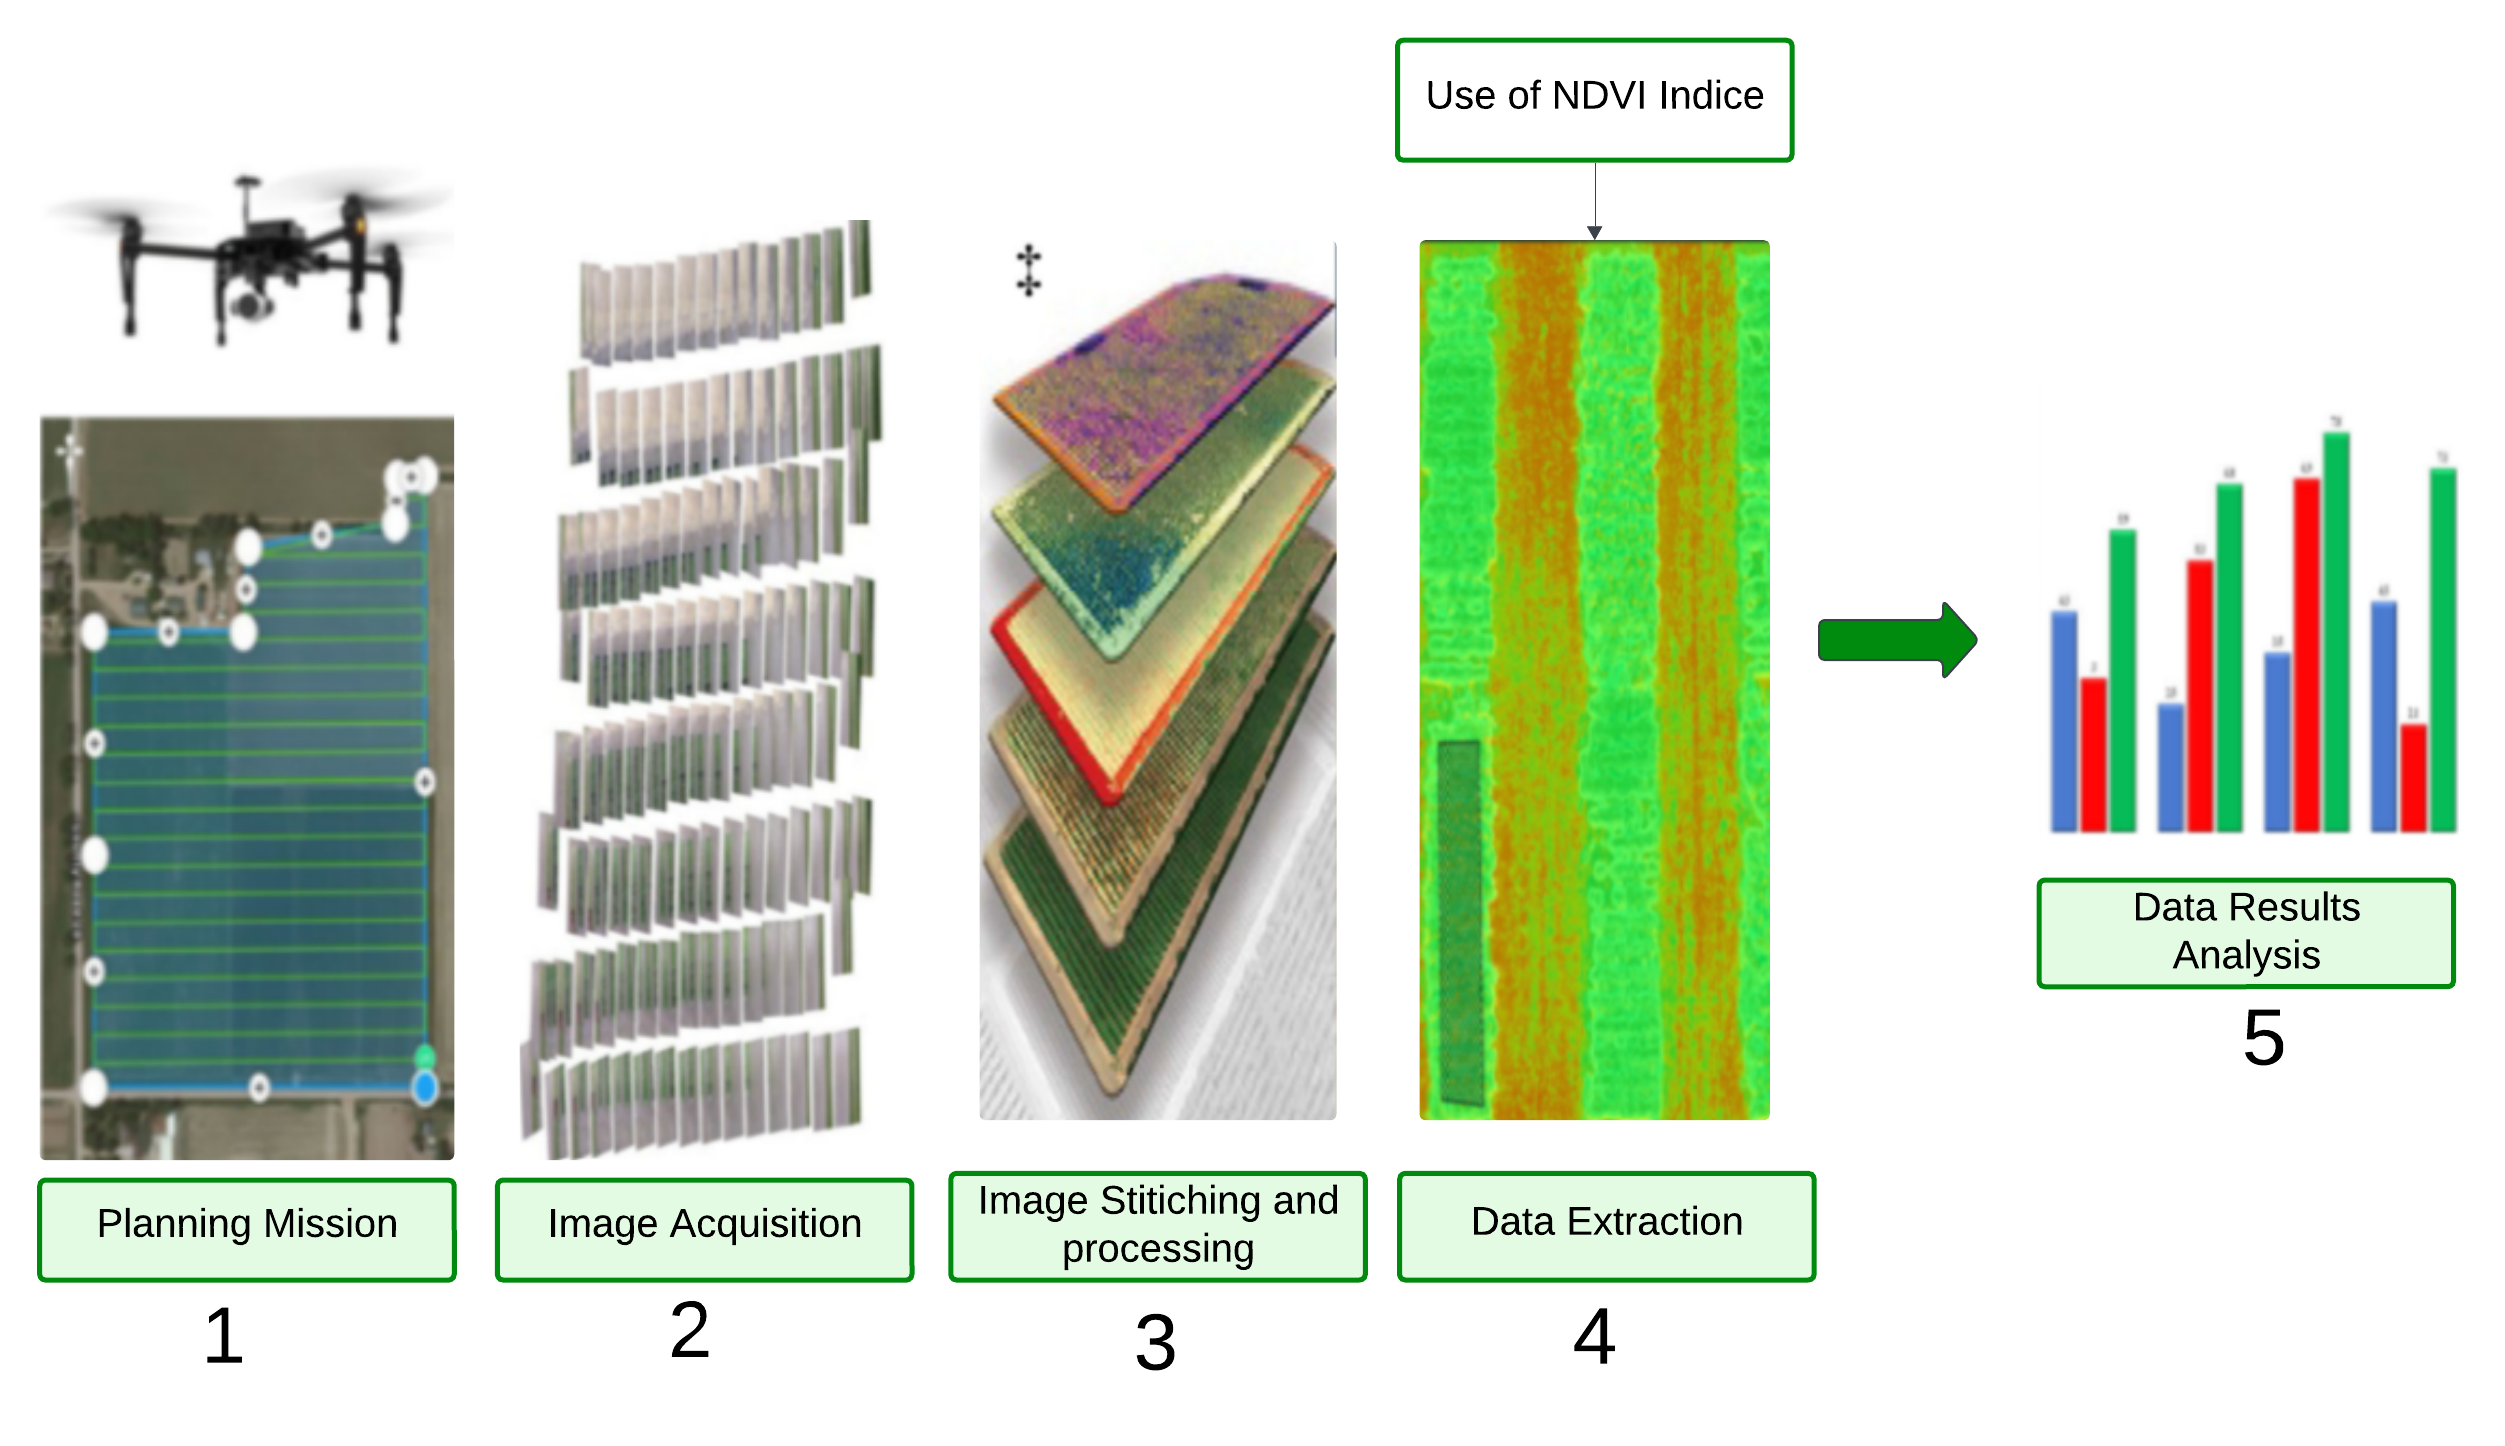
\includegraphics[width=0.9\textwidth]{chapters/chapter3/images/Figure06.png}
    \caption{Architecture diagram of a Few-shot Learning-based network \parencite{alharbi2023wheat}.}
    \label{fig:Few-shot}
\end{figure}


\textbf{Lightweight \gls{abb:cnn}s for efficient classification \parencite{fang2023lightweight}:} Introduced a lightweight multiscale \gls{abb:cnn} model optimized for mobile and edge computing applications. By integrating Inception modules with residual blocks and attention mechanisms like Convolutional Block Attention Model (CBAM) (More details in Appendix~\ref{app:annexA}) and Efficient Channel Attention (ECA), the model enhanced feature extraction while reducing computational costs, achieving 98.78\% accuracy on wheat disease classification tasks​. Likewise, \parencite{jouini2023wheat} proposed a deep learning approach using MobileNetV2 and EfficientNet variants to build a lightweight yet accurate \gls{abb:cnn}-based model for wheat leaf disease detection in smart agriculture, achieving 94\% test accuracy. 


The studies are complementary as they address different challenges in wheat disease classification. After reviewing various approaches adopted in the literature, we constructed a taxonomy that summarizes the main strategies employed in this field, as illustrated in Figure~\ref{fig:Figure0001}. This taxonomy includes transfer learning, hybrid models, custom \gls{abb:cnn} architectures, few-shot learning, lightweight \gls{abb:cnn}s, and attention mechanisms. Transfer learning helps overcome limited data by leveraging pre-trained models, while hybrid models combine deep learning and traditional machine learning to enhance performance. Custom and task-specific \gls{abb:cnn}s are tailored to the unique features of wheat diseases, improving accuracy. Few-shot learning enables effective classification with minimal labeled data, and lightweight \gls{abb:cnn}s optimize real-time detection for mobile and edge devices, balancing performance with computational efficiency. Each approach targets a specific problem, enhancing the overall classification process.

\begin{figure}[H]
    \centering
    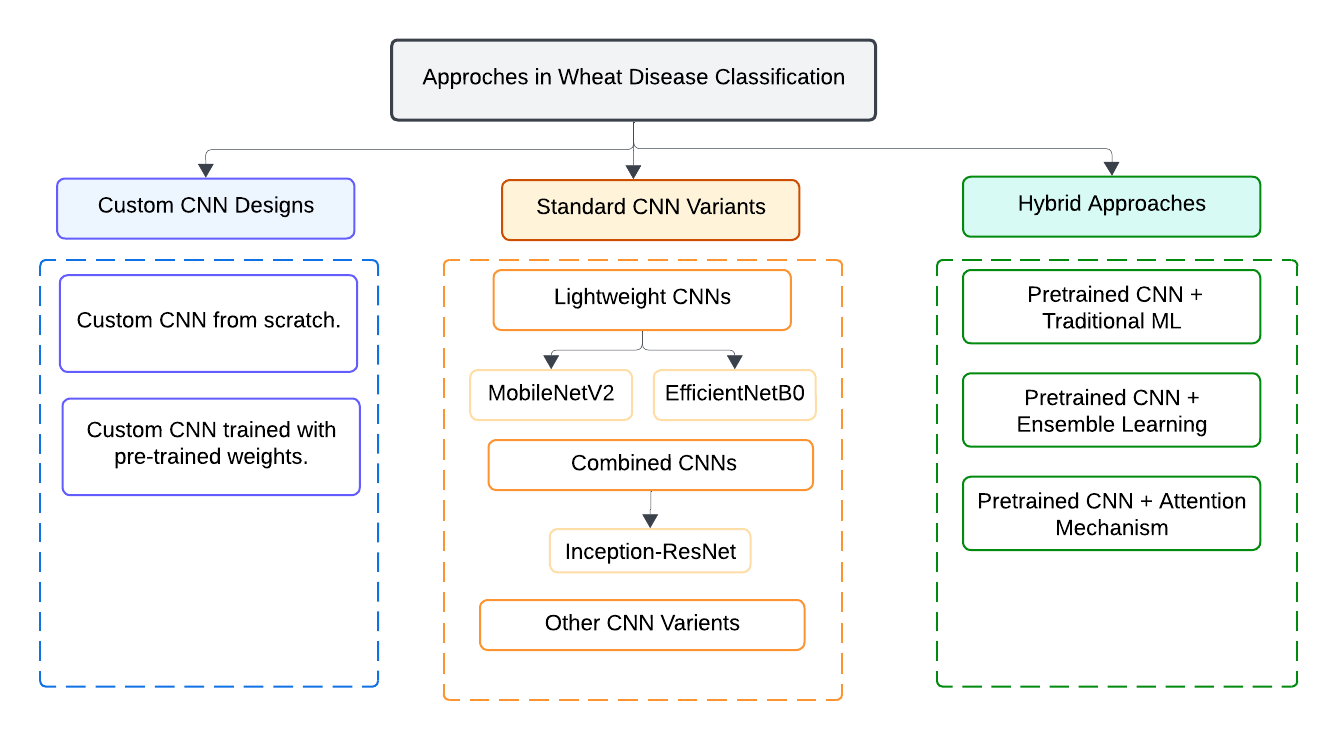
\includegraphics[width=1.1\textwidth]{chapters/chapter3/images/Figure09.png}
    \caption{Taxonomy of approaches for classifying wheat diseases.}
    \label{fig:Figure0001}
\end{figure}


\subsection{Core limitations and research gaps in wheat disease identification}
Deep learning has shown great promise in automating wheat disease detection, offering timely and precise solutions for sustainable agriculture. However, key challenges still limit its widespread adoption.

Based on the previously discussed studies, various approaches have been explored for wheat disease classification, ranging from transfer learning using pre-trained convolutional neural networks (\gls{abb:cnn}s) to the development of custom architectures tailored specifically for disease classification tasks. The proposed models for wheat disease classification that detect five or fewer disease classes generally achieve accuracies of 99\% or higher. However, models aiming to detect more than five classes tend to achieve lower accuracies, typically below 98\%, highlighting the challenge of achieving high accuracy when dealing with more complex classification tasks.

Additionally, the number of disease classes addressed in most proposed models for wheat detection remains limited compared to the actual variety of diseases observed in the field, with a maximum of five classes, primarily due to the difficulty of manual annotation and the high computational resources required to train models on larger, more diverse datasets. Although several public datasets for wheat disease classification are available, such as those on Kaggle, these sources often contain low-quality images, inconsistent labeling, or irrelevant data, which can hinder model training and performance. This necessitates manual cleaning and preprocessing of the datasets before they can be effectively utilized, increasing the time and effort needed for research.

Moreover, the performance of these models is often affected by inconsistencies in image data. Therefore, diversifying image data is crucial; photos should be taken under varying lighting conditions, such as on sunny and cloudy days, and from different distances, including both close-up and wider shots. Creating a custom dataset by selecting diverse images from different public datasets is important to ensure this variability and improve model robustness.

Beyond dataset issues, several structural and architectural limitations remain. Most current models use a single-stage classification pipeline that attempts to identify all classes in one pass. This approach can be inefficient, especially when simple distinctions (e.g., healthy vs. diseased) could be resolved earlier using lightweight inference mechanisms. The lack of hierarchical or multi-stage classification pipelines presents an opportunity for improvement in computational efficiency and deployment readiness.

Furthermore, few models explicitly address deployment constraints such as low computational power, memory limitations, or real-time processing requirements, which are crucial for applications in edge computing or mobile agricultural tools used directly in the field. The absence of design considerations for lightweight architectures and early-exit strategies limits the practical applicability of many existing solutions.

Another significant limitation is the lack of evaluation on real-world field images that exhibit high variability in terms of background, illumination, occlusion, and resolution. While many models achieve excellent performance on curated datasets, their generalization to uncontrolled field conditions remains underexplored. Robustness under such conditions is essential for real-life adoption by farmers and agronomists.

Finally, although attention mechanisms and hybrid models have been proposed in recent literature, few studies explicitly quantify the trade-offs between accuracy and computational cost in multi-class settings, especially when scaling up to cover a wider range of diseases.


\section{Conclusion}
While deep learning has shown strong potential in wheat disease detection, a major limitation across current studies is the restricted number of disease classes addressed often no more than five. This narrow scope limits the practical applicability of these models in real agricultural environments, where a wider range of diseases must be identified accurately. The difficulty of collecting and annotating diverse, high-quality images, along with the computational cost of training on large-scale multi-class datasets, remains a significant barrier. Additionally, many existing models struggle to maintain high accuracy when scaled to include more disease categories.

These challenges highlight the need for systems capable of handling a greater number of classes without compromising accuracy. In the next chapter, we present the design and implementation of our proposed solution, which is specifically developed to support accurate multi-class classification and improved generalization to real-world conditions.